\documentclass[9pt,twocolumn,twoside]{osajnl}

\journal{ao} % Choose journal (ao, ol, josaa, josab)

\setboolean{shortarticle}{false} % true = letter, false = research article

\title{\LaTeX\ template for preparing an article for submission to OSA journals \emph{Applied Optics}, \emph{Optics Letters}, \emph{JOSA-A} and \emph{JOSA-B}}

\author[1,2,3]{Author One}
\author[2,*]{Author Two}
\author[1]{Author Three}

\affil[1]{Publications Department, OSA-The Optical Society, 2010 Massachusetts Avenue NW, Washington D.C., 20036}
\affil[2]{School of Science, University of Technology, 2000 J St. NW, Washington DC, 20036}
\affil[3]{School of Optics, University of Technology, 2000 J St. NW, Washington DC, 20036}

\affil[*]{Corresponding author: email@my-email.com}

\dates{Compiled \today}



\doi{\url{http://dx.doi.org/10.1364/ao.XX.XXXXXX}}

\begin{abstract}
This template can be used to prepare a research article for submission to OSA’s journals \emph{Applied Optics}, \emph{JOSA A}, \emph{JOSA B}, and \emph{Optics Letters}. For \emph{Optics Letters}, you will need to select \texttt{$\setminus$setboolean\{shortarticle\}\{true\}}. Note that this template can be run from your own \TeX\ system or within the cloud-based \href{https://www.overleaf.com}{Overleaf} system (formerly writeLaTeX). For \emph{Optics Letters} select \setboolean{shortarticle}{true} to get a one-column abstract.
\end{abstract}

\setboolean{displaycopyright}{true}

\begin{document}

\maketitle
\thispagestyle{fancy}
\ifthenelse{\boolean{shortarticle}}{\abscontent}{}

\section{Introduction}

This template is designed to assist with creating a two-column research article or letter to submit to \emph{Applied Optics}, \emph{JOSA A}, \emph{JOSA B}, and \emph{Optics Letters}. See the OSA's \href{http://www.opticsinfobase.org/submit/style/}{Style Guide} and \href{http://www.opticsinfobase.org/submit/templates/}{Manuscript Templates} pages for more details.

If you have a question while using this template on \href{https://www.overleaf.com}{Overleaf}, please use the help menu (``?'') on the top bar to search for help or ask us a question using the option in the lower right of the editor.

\section{Examples of Article Components}
\label{sec:examples}

The sections below show examples of different article components.

\section{Figures and Tables}

It is not necessary to place figures and tables at the back of the manuscript. Figures and tables should be sized as they are to appear in the final article. Do not include a separate list of figure captions and table titles.

Figures and Tables should be labelled and referenced in the standard way using the \verb|\label{}| and \verb|\ref{}| commands.

\subsection{Sample Figure}

Figure \ref{fig:false-color} shows an example figure.

\begin{figure}[htbp]
\centering
\fbox{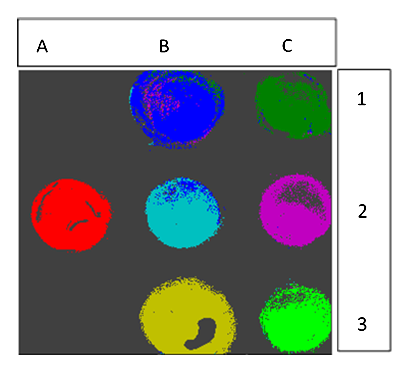
\includegraphics[width=\linewidth]{sample}}
\caption{False-color image, where each pixel is assigned to one of seven reference spectra.}
\label{fig:false-color}
\end{figure}

\subsection{Sample Table}

Table \ref{tab:shape-functions} shows an example table.

\begin{table}[htbp]
\centering
\caption{\bf Shape Functions for Quadratic Line Elements}
\begin{tabular}{ccc}
\hline
local node & $\{N\}_m$ & $\{\Phi_i\}_m$ $(i=x,y,z)$ \\
\hline
$m = 1$ & $L_1(2L_1-1)$ & $\Phi_{i1}$ \\
$m = 2$ & $L_2(2L_2-1)$ & $\Phi_{i2}$ \\
$m = 3$ & $L_3=4L_1L_2$ & $\Phi_{i3}$ \\
\hline
\end{tabular}
  \label{tab:shape-functions}
\end{table}

\section{Sample Equation}

Let $X_1, X_2, \ldots, X_n$ be a sequence of independent and identically distributed random variables with $\text{E}[X_i] = \mu$ and $\text{Var}[X_i] = \sigma^2 < \infty$, and let
\begin{equation}
S_n = \frac{X_1 + X_2 + \cdots + X_n}{n}
      = \frac{1}{n}\sum_{i}^{n} X_i
\label{eq:refname1}
\end{equation}
denote their mean. Then as $n$ approaches infinity, the random variables $\sqrt{n}(S_n - \mu)$ converge in distribution to a normal $\mathcal{N}(0, \sigma^2)$.

\section{Sample Algorithm}

Algorithms can be included using the commands as shown in algorithm \ref{alg:euclid}.

\begin{algorithm}
\caption{Euclid’s algorithm}\label{alg:euclid}
\begin{algorithmic}[1]
\Procedure{Euclid}{$a,b$}\Comment{The g.c.d. of a and b}
\State $r\gets a\bmod b$
\While{$r\not=0$}\Comment{We have the answer if r is 0}
\State $a\gets b$
\State $b\gets r$
\State $r\gets a\bmod b$
\EndWhile\label{euclidendwhile}
\State \textbf{return} $b$\Comment{The gcd is b}
\EndProcedure
\end{algorithmic}
\end{algorithm}

\section{Supplementary Material}

Consult the \href{https://www.osapublishing.org/submit/style/multimedia.cfm}{Author Guidelines for Supplementary Materials in OSA Journals} for details on accepted types of materials and instructions on how to cite them. All materials must be associated with a figure, table, or equation or be referenced in the results section of the manuscript.

2D and 3D image files and video must be labeled “Visualization,” not “Movie,” “Video,” “Figure,” etc. Machine-readable data (for example, csv files) must be labeled  “Data File.”  Number data files and visualizations consecutively, e.g., “Visualization 1, Visualization 2, etc.”. Such items should be mentioned in the text as either “Dataset” or “Code,” as appropriate, and also be cited in the references list. For example, see Dataset 1 (Ref. [1])  and Code 1 (Ref. [2]). Here are two examples:

Sample Dataset Citation

1. T. Ireno and R. Tadaa, "Chemical and mineral compositions of sediments from ODP Site 127-797" (Geological Institute, University of Tokyo, 2009), http://dx.doi.org/10.1594/PANGAEA.726855.

Sample Code Citation

2. Zima Engineering, ZIMA-CAD-Parts: Application for management of CAD files and projects (version 0.5.0-beta1) [software] (2013), http://sourceforge.net/projects/zima-cad-parts/.

\section*{Funding Information}

\textbf{Funding.} National Science Foundation (NSF) (1263236, 0968895, 1102301); The 863 Program (2013AA014402).

\section*{Acknowledgments}

\textbf{Acknowledgment.} Formal funding declarations should not be included in the acknowledgments but in a Funding Information section as shown above. The acknowledgments may contain information that is not related to funding:

The authors thank H. Haase, C. Wiede, and J. Gabler for technical support.

\section*{References}

Note that \emph{Optics Letters} does not include journal article titles or full page ranges in the published article. Only the first page is required. However, a fifth informational-only page containing the full references should be included. The informational page does not count toward the length restriction.

\bigskip
\noindent Add citations manually or use BibTeX. See \cite{Zhang:14}.

% Bibliography
\bibliography{sample}

%Manual citation list
%\begin{thebibliography}{1}
%\bibitem{Zhang:14}
%Y.~Zhang, S.~Qiao, L.~Sun, Q.~W. Shi, W.~Huang, %L.~Li, and Z.~Yang,
 % \enquote{Photoinduced active terahertz metamaterials with nanostructured
  %vanadium dioxide film deposited by sol-gel method,} Opt. Express \textbf{22},
  %11070--11078 (2014).
%\end{thebibliography}

\end{document}
